\documentclass[../HAFiscal]{subfiles}
\begin{document}

\FloatBarrier
\section{Robustness}
\label{sec:robustness}

\begin{table}[th]
\begin{center}
\begin{tabular}{lc|cccccc} 
	\toprule
	& & \multicolumn{2}{c}{Dropout} & \multicolumn{2}{c}{Highschool} & \multicolumn{2}{c}{College} \\ \midrule 
	 & Splurge & $\beta$ & $\nabla$ & $\beta$ & $\nabla$ & $\beta$ & $\nabla$ \\ \midrule 
	$\gamma = 1.0$ (baseline) & 0.314 & 0.799 & 0.228 & 0.937 & 0.066 & 0.985 & 0.012 \\ 
	$\gamma = 1.5$ & 0.310 & 0.667 & 0.243 & 0.894 & 0.115 & 0.976 & 0.022 \\
	$\gamma = 2.0$ & 0.307 & 0.551 & $0.5^*$ & 0.834 & 0.181 & 0.963 & 0.036 \\
	$\gamma = 3.0$ & 0.304 & 0.345 & $0.3^*$ & 0.671 & 0.364 & 0.917 & 0.087 
	\\ \bottomrule 
\end{tabular}
\end{center}
\caption{Robustness exercise: Estimating the Splurge, and $(\beta,\nabla)$ for each education group for different values of risk aversion, $\gamma$. $*$ indicates a value that is fixed in the estimation --- this is necessary in some cases to prevent the estimation procedure from trying negative values for the discount factor of some type.}
\label{tab:robustness_gamma}
\end{table}



\begin{figure}[th]
\begin{center}
	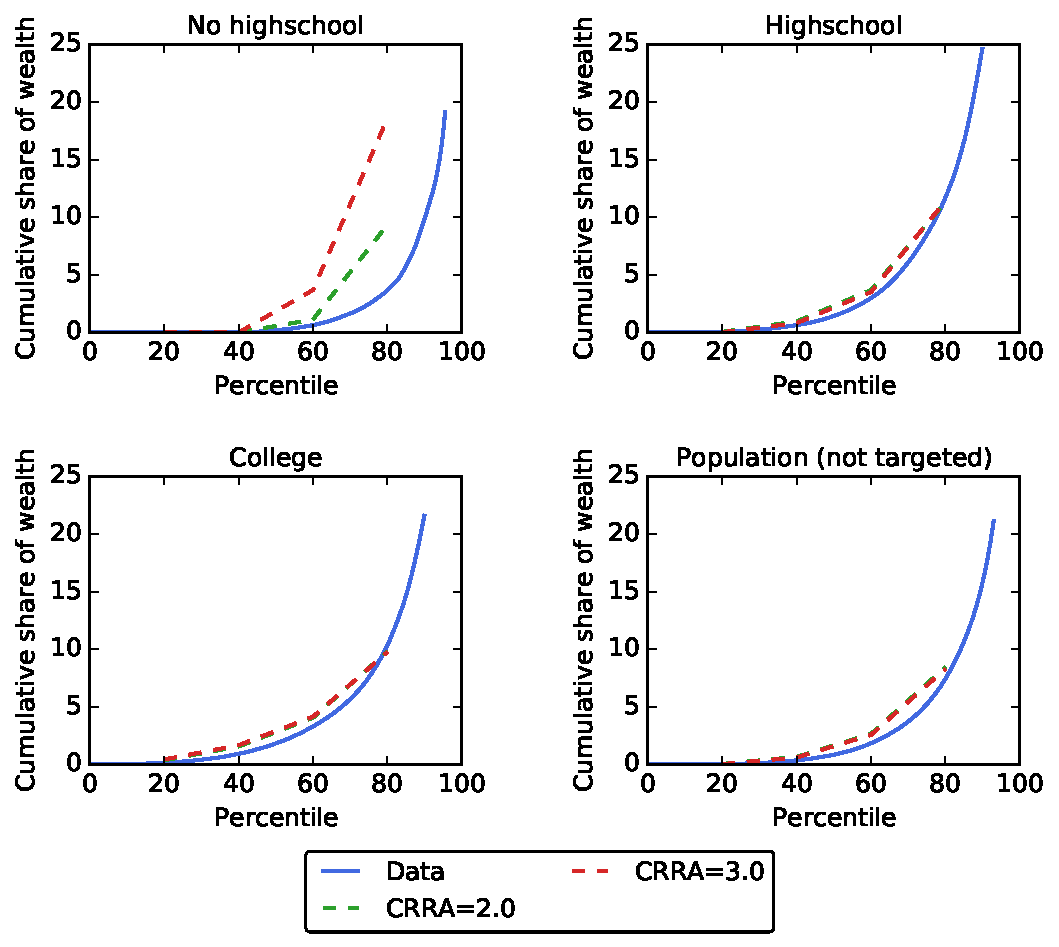
\includegraphics[width=.9\textwidth]{../Figures/LorenzPoints_robustness.pdf}
	\caption{Distributions of liquid wealth within each educational group and for the whole population from the 2004 Survey of Consumer Finance and from the estimated model for different values of risk aversion, $\gamma$.}
	\label{fig:LorenzPts_robustness}
\end{center}
\end{figure}


\end{document}	